% Options for packages loaded elsewhere
\PassOptionsToPackage{unicode}{hyperref}
\PassOptionsToPackage{hyphens}{url}
%
\documentclass[
]{article}
\usepackage{lmodern}
\usepackage{amssymb,amsmath}
\usepackage{ifxetex,ifluatex}
\ifnum 0\ifxetex 1\fi\ifluatex 1\fi=0 % if pdftex
  \usepackage[T1]{fontenc}
  \usepackage[utf8]{inputenc}
  \usepackage{textcomp} % provide euro and other symbols
\else % if luatex or xetex
  \usepackage{unicode-math}
  \defaultfontfeatures{Scale=MatchLowercase}
  \defaultfontfeatures[\rmfamily]{Ligatures=TeX,Scale=1}
\fi
% Use upquote if available, for straight quotes in verbatim environments
\IfFileExists{upquote.sty}{\usepackage{upquote}}{}
\IfFileExists{microtype.sty}{% use microtype if available
  \usepackage[]{microtype}
  \UseMicrotypeSet[protrusion]{basicmath} % disable protrusion for tt fonts
}{}
\makeatletter
\@ifundefined{KOMAClassName}{% if non-KOMA class
  \IfFileExists{parskip.sty}{%
    \usepackage{parskip}
  }{% else
    \setlength{\parindent}{0pt}
    \setlength{\parskip}{6pt plus 2pt minus 1pt}}
}{% if KOMA class
  \KOMAoptions{parskip=half}}
\makeatother
\usepackage{xcolor}
\IfFileExists{xurl.sty}{\usepackage{xurl}}{} % add URL line breaks if available
\IfFileExists{bookmark.sty}{\usepackage{bookmark}}{\usepackage{hyperref}}
\hypersetup{
  pdftitle={Can we predict house prices using known features of each house and a supervised learning approach?},
  pdfauthor={Florence Galliers},
  hidelinks,
  pdfcreator={LaTeX via pandoc}}
\urlstyle{same} % disable monospaced font for URLs
\usepackage[margin=1in]{geometry}
\usepackage{graphicx,grffile}
\makeatletter
\def\maxwidth{\ifdim\Gin@nat@width>\linewidth\linewidth\else\Gin@nat@width\fi}
\def\maxheight{\ifdim\Gin@nat@height>\textheight\textheight\else\Gin@nat@height\fi}
\makeatother
% Scale images if necessary, so that they will not overflow the page
% margins by default, and it is still possible to overwrite the defaults
% using explicit options in \includegraphics[width, height, ...]{}
\setkeys{Gin}{width=\maxwidth,height=\maxheight,keepaspectratio}
% Set default figure placement to htbp
\makeatletter
\def\fps@figure{htbp}
\makeatother
\setlength{\emergencystretch}{3em} % prevent overfull lines
\providecommand{\tightlist}{%
  \setlength{\itemsep}{0pt}\setlength{\parskip}{0pt}}
\setcounter{secnumdepth}{5}
\usepackage{booktabs}
\usepackage{longtable}
\usepackage{array}
\usepackage{multirow}
\usepackage{wrapfig}
\usepackage{float}
\usepackage{colortbl}
\usepackage{pdflscape}
\usepackage{tabu}
\usepackage{threeparttable}
\usepackage{threeparttablex}
\usepackage[normalem]{ulem}
\usepackage{makecell}
\usepackage{xcolor}

\title{Can we predict house prices using known features of each house and a
supervised learning approach?}
\author{Florence Galliers}
\date{18/10/2020}

\begin{document}
\maketitle

{
\setcounter{tocdepth}{2}
\tableofcontents
}
\newpage

\hypertarget{background}{%
\section{Background:}\label{background}}

House prices are an important part of the economy and usually reflect
trends in it. They can be influenced by the physical condition of the
house and by other attributes such as location (Bin
\protect\hyperlink{ref-bin2004prediction}{2004}). Prices are important
for homeowners, prospective buyers and estate agents. Prediction methods
could help lead to more informed decisions to each of these
stakeholders. Gao et al. (\protect\hyperlink{ref-gao2019location}{2019})
suggest that prediction models may be useful for narrowing down the
range of available houses for prospective buyers and allowing sellers to
predict optimal times to list their houses on the market. Prediction
accuracy would be important in all of these situations as inaccurate
models would not be trusted by their users.

Something else to take into account is that it may be difficult for
prospective buyers to visualise how square footage measurements of a
house are calculated or how this measurement translates into physical
size if they have not visited the house themselves. Buyers therefore
rely on factors such as the number of bedrooms, bathrooms or house age
to get an idea of the value of the house. This analysis will focus on
which features of a house have the \textbf{largest influence} on the
prediction of house prices. This report does not look at the effect of
time on house prices. It is already well known that house prices tend to
increase year on year (Alfiyatin et al.
\protect\hyperlink{ref-alfiyatin2017modeling}{2017}).

In most countries there is some form of house price index that measures
changes in prices (Lu et al.
\protect\hyperlink{ref-lu2017hybrid}{2017}). This contains a summary of
all transactions that take place but not the individual features of each
house sold, therefore it cannot be used to make predictions of house
price.

Many house price prediction models have been created using machine
learning methods. The hedonic price model is the most extensively
researched and uses regression methods (Gao et al.
\protect\hyperlink{ref-gao2019location}{2019}). Hedonic models assume
that the value of a house is reflected by a set of attributes (Bin
\protect\hyperlink{ref-bin2004prediction}{2004}). The goal of a
regression approach is to build an equation which defines y, the
dependent variable as a function of the x variable(s). This equation can
then be used for prediction of y when given unseen values of x. Machine
learning methods use data in a `training set' to build a model, this
model is then used to make predictions on an unseen `test set' of data.
The accuracy of models can be calculated by taking the predicted values
from the actual values.

\hypertarget{objectives}{%
\subsection{Objectives:}\label{objectives}}

\begin{itemize}
\tightlist
\item
  Understand which attributes of houses can be used to effectively
  construct a prediction model for house price.
\item
  Minimize the differences between predicted and actual house prices by
  using model selection to choose the most accurate model.
\end{itemize}

\hypertarget{data}{%
\section{Data:}\label{data}}

\hypertarget{data-description}{%
\subsection{Data Description}\label{data-description}}

The dataset chosen for this analysis contains the house sale price, in
US dollars, along with attributes of each house such as number of
bedrooms, number of bathrooms, etc. The houses were all sold in
Washington in 2014, a state in the Northwest of the USA. There were 4600
observations with 17 variables in the original data set downloaded from
{[}Kaggle{]} (\url{https://www.kaggle.com/shree1992/housedata}).
Although the dataset was from 2014, it was particularly interesting
because it contained a large amount of information and an interesting
selection of variables. A more recent data set, or one from the UK could
not be found, and so the analysis went ahead with this data set.

\hypertarget{data-preparation-and-exploration}{%
\subsection{Data Preparation and
Exploration}\label{data-preparation-and-exploration}}

The first task was preparing and cleaning the dataset. This served two
purposes, firstly to get to know the different variables in the data and
existing patterns or correlations between them and secondly to carry out
feature selection. Variables that contained a majority missing data,
those with constant variables (e.g.~Country contained the value USA for
all observations) and the date column were removed. Any observations in
which price was equal to zero were removed. The cleaned dataset was
exported ready for use in the main analysis. This cleaned data set
contained 4492 observations and 11 variables (Table 1). Some alterations
were made to existing variables, these are listed in the descriptions of
table 1 alongside the variable.

\textbf{Table 1}: Description of all variables present in the cleaned
dataset and explanations of how they were calculated if they have been
altered from the original dataset

\begin{tabular}{|>{}l|>{\raggedright\arraybackslash}p{12cm}|}
\hline
\textbf{Variable} & \textbf{Description of Variable}\\
\hline
\textbf{price} & House sale price in thousands of US dollars, the original data was divided by 1000 to give this value, numeric\\
\hline
\textbf{bedrooms} & Number of bedrooms, numeric\\
\hline
\textbf{bathrooms} & Number of bathrooms, numeric\\
\hline
\textbf{sqft\_living} & Area of house in square feet, numeric\\
\hline
\textbf{sqft\_lot} & Area of whole housing lot in square feet, numeric\\
\hline
\textbf{floors} & Number of floors in the house, numeric\\
\hline
\textbf{condition} & Condition of house from 1 to 5, numeric\\
\hline
\textbf{if\_basement} & 1 = if house has a basement, 0 = if house has no basement, this was originally showing the size of the basement, but not all houses had basements so it was changed to binary\\
\hline
\textbf{house\_age} & House Age in years, calculated by 2014 minus the year the house was built\\
\hline
\textbf{if\_renovated} & 1 = if house has been renovated, 0 = if no renovation, again this was originally showing the year of renovation however not all houses had been renovated and so it was changed to binary\\
\hline
\textbf{city} & Factor variable (32 levels) giving location of house to the nearest city in Washington, USA, any city that had less than 10 houses was removed\\
\hline
\end{tabular}

\hypertarget{data-visualisation}{%
\subsection{Data Visualisation}\label{data-visualisation}}

The cleaned data set was explored to look for any correlations between
variables (Figure 1). Spearmans correlation was used to produce a
correlation coefficient giving the strength of the linear relationship
between two variables. This method of correlation was chosen as not all
of the relationships looked entirely linear when they were plotted. The
dependent variable (price) had a positive correlation with house size,
number of bathrooms and number of bedrooms. The strongest relationship
seen was between sqft\_living and number of bathrooms. It is interesting
to note that the only non significant correlation involving price is
between price and house age. Multicollinearity occurs when two variables
are heavily intercorrelated in a regression model and it can lead to
less accurate predictions, the presence or absence of this in the data
will be explored further on in the methods.

\textbf{Figure 1}: A correlation map showing the correlations between
variables according to spearmans correlation (excluding city,
if\_basement and if\_renovated), the colours represent strength of
correlation, the crosses show where the correlation is not significant.

\includegraphics[width=0.6\linewidth]{C7081-report_files/figure-latex/Correlation Plot-1}

\hypertarget{methods}{%
\section{Methods}\label{methods}}

A supervised learning approach was chosen throughout this analysis. In a
supervised learning approach there is a continuous response variable of
which predictions are to be made, and a number of predictor variables.
In all the approaches tried house price was a quantitative variable.

The dataset was split randomly into two parts, a training set containing
80\% of the observations and a test set containing the remaining 20\%.
The training set was used to train all of the models and the test set to
assess accuracy of the models. This split was completed using the
\emph{sample} function, which took a random sample of 80\% of the data
without replacement to act as the train data, everything remaining was
the test set.

\hypertarget{linear-regression}{%
\subsection{Linear Regression}\label{linear-regression}}

Firstly, a simple linear regression model was created using price as the
dependent variable (y) and square foot living area (sqft\_living) as the
independent variable (x). Sqft\_living was chosen because it was shown
to be the most correlated variable to house price in the exploratory
data analysis. A simple linear regression model uses the \emph{lm()}
function. This linear regression takes a model with equation

price = B0 + B1(sqft\_living) + E

and estimates coefficients which produce a line of best fit, minimising
the difference between predicted and actual values. This type of simple
linear regression is known as ordinary least squares. In the equation
above, B0 is the intercept, B1 is the coefficient produced by the model
and E is the error term.

This simple model was then expanded to allow all the other variables in
the dataset to act as predictor variables, this is known as multiple
linear regression. The model output showed that 17 of these variables
had a significant impact (P\textless0.05) on the price. The coefficients
and P values of each of these variables are shown below.

\textbf{Table 2}: Names and Coefficient estimates of only the variables
that showed significant P-values in the multiple linear regression model
involving all predictor variables.

\begin{tabular}{|>{}l|r|>{}r|}
\hline
  & Coef Estimates & P-Value\\
\hline
(Intercept) & -300.0848039 & 0.0004652\\
\hline
bedrooms & -58.3531453 & 0.0000065\\
\hline
bathrooms & 68.2541014 & 0.0012979\\
\hline
sqft\_living & 0.2609683 & 0.0000000\\
\hline
condition & 36.6402055 & 0.0231854\\
\hline
if\_basement1 & -58.8254709 & 0.0091500\\
\hline
house\_age & 1.0007524 & 0.0342776\\
\hline
\cellcolor{grey}{cityBellevue} & \cellcolor{grey}{402.9644709} & \cellcolor{grey}{0.0000000}\\
\hline
\cellcolor{grey}{cityIssaquah} & \cellcolor{grey}{192.8171552} & \cellcolor{grey}{0.0023546}\\
\hline
\cellcolor{grey}{cityKent} & \cellcolor{grey}{192.0829810} & \cellcolor{grey}{0.0023943}\\
\hline
\cellcolor{grey}{cityKirkland} & \cellcolor{grey}{286.7290160} & \cellcolor{grey}{0.0000059}\\
\hline
\cellcolor{grey}{cityMedina} & \cellcolor{grey}{1191.9241550} & \cellcolor{grey}{0.0000000}\\
\hline
\cellcolor{grey}{cityMercerisland} & \cellcolor{grey}{529.6076728} & \cellcolor{grey}{0.0000000}\\
\hline
\cellcolor{grey}{cityRedmond} & \cellcolor{grey}{243.3809709} & \cellcolor{grey}{0.0000647}\\
\hline
\cellcolor{grey}{citySammamish} & \cellcolor{grey}{217.8271899} & \cellcolor{grey}{0.0008843}\\
\hline
\cellcolor{grey}{citySeattle} & \cellcolor{grey}{313.5117092} & \cellcolor{grey}{0.0000000}\\
\hline
\cellcolor{grey}{cityShoreline} & \cellcolor{grey}{158.5865198} & \cellcolor{grey}{0.0215383}\\
\hline
\cellcolor{grey}{cityWoodinville} & \cellcolor{grey}{143.9101433} & \cellcolor{grey}{0.0460584}\\
\hline
\end{tabular}

It should be noted that \emph{if\_basement}, \emph{if\_renovated} and
\emph{city} were all factor variables, and so when they were fit into a
model, they were converted into dummy variables, with one for each
factor level. This is why some of the variables selected above are not
the same as those variables shown in the cleaned data set. This also
raises the idea that location has a large influence on house price as 11
of the variables shown above are all dummy variables originating from
\emph{city}.

Multicollinearity was also explored from the multiple linear model. The
variance inflation factors (VIF) for each variable was calculated which
shows how much of the variance of the regression coefficient is inflated
due to any multicollinearity in the model. None of the VIF were above 5,
with the highest being \emph{bathrooms} at 3.3, and so there was no
problematic collinearity indicated. This was carried out using the
\emph{vif()} function in the \emph{car} package.

Polynomial models of regression were trialed but they did not improve
RMSE results, so this approach was not looked into further. The
relationship between sqft\_living and price looked to be linear in the
exploratory data analysis so this was not a surprising development.

\hypertarget{variable-selection-methods}{%
\subsection{Variable Selection
Methods}\label{variable-selection-methods}}

To look further into which variables were most influential on price,
variable selection methods were explored. Best subset selection is a
method that finds the best combinations of predictors that produce the
best fit in terms of squared error. Forward stepwise selection is
slightly different as it starts with no variables and one by one adds
the variable which gives the smallest increase in squared error.
Backward stepwise selection follows the same idea as forward selection
but it starts with a full model, and iteratively removes variables until
it leaves a one variable model with the lowest mean squared error.

In best subset selection, cross-validation was used to choose among
variables of differing sizes. This is a direct method of estimating test
error. A model with 15 variables had the lowest cross-validation error.
These variables were extracted and a linear model created containing
only them. This linear model had a lower MSE than the simple linear
model with just one variable, but was higher, therefore less accurate
than the multiple linear model created with just

If we had used R2 statistics to assess the models, we would always end
up with a model containing all of the variables as the `best' one. In
this analysis direct methods of test error estimation were used, however
as an alternative, adjusted R2, CP or BIC criterion may have been used
to indirectly estimate the test error. Validation set approach was also
take to estimate test error, this gave a model with many more variables
and so it was decided that cross-validation was the most appropriate
method to use to help narrow down the variables to the most influential.

The validation error at different model sizes for the three kinds of
variable selection are shown in Figure 2, this also includes the
cross-validation error for best-subset selection. Forward and backward
selection yielded almost identical results to each other with only a one
variable difference to best-subset selection. The specific variables
selected from best-subset selection were also very similar to the ones
that showed a significant effect in the multiple linear model, with only
one variable different. Forward and backward subset selection methods
gave lower MSE results than best-subset selection. Figure 2 shows that
all of these methods produce extremely similar results.

\newpage

\textbf{Figure 2}: The Validation and Cross Validation Error plots for
best-subset, forward and backward selection.
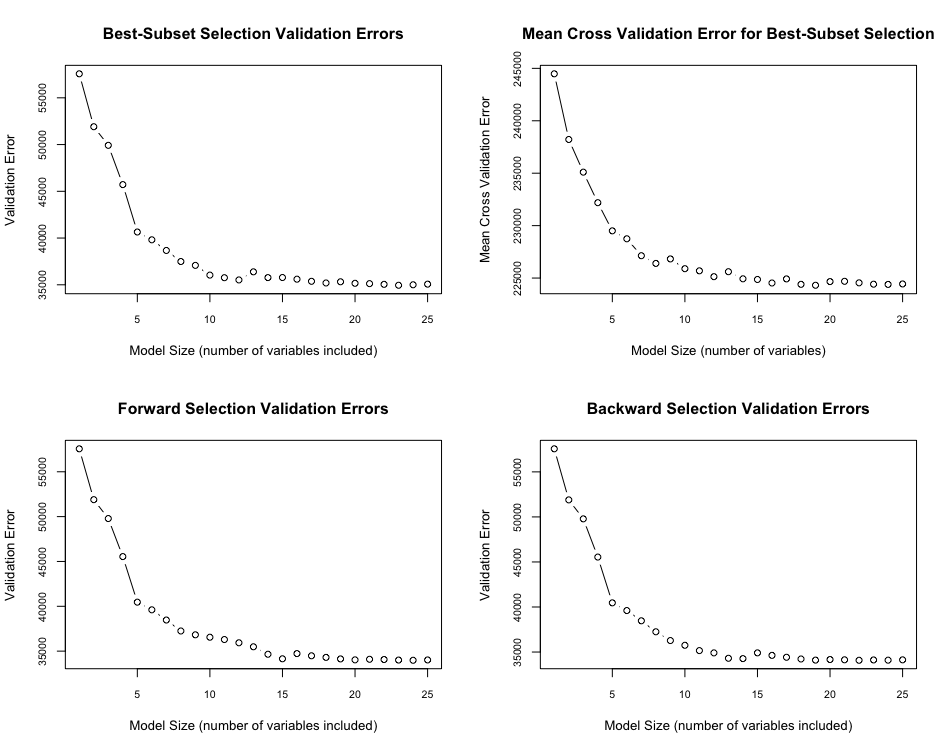
\includegraphics{/Users/florentinagalliers/Google Drive/Harper/1-C7081/Asssesment/github-C7081/C7081-assessment/validation-error-plot.png}

\hypertarget{ridge-regression-and-lasso}{%
\subsection{Ridge Regression and
LASSO}\label{ridge-regression-and-lasso}}

Ridge Regression and the LASSO are both shrinkage methods. In the above
variable selection methods, only a subset of predictors are used. In
shrinkage methods all of the predictors are included in the model but
the coefficient estimates are constrained towards zero, this can help to
reduce variance.

Ridge Regression utilises L2 regularisation, this adds a penalty to the
coefficients that is equal to the square of the coefficients. Lambda is
a tuning parameter, as its magnitude increases, the shrinkage penalty
has more of an impact and the coefficient estimates will be closer to
zero. Selecting the right value of lambda is very important, in this
analysis it was selected using cross-validation. If lambda = 0, this
method would be identical to ordinary least squares. Ridge regression
does however always include all of the variables in the data set, this
can lead to problems with interpretation.

LASSO is another coefficient shrinkage technique in which the L0 norm is
replaced with the L1 norm. LASSO stands for Least Absolute Shrinkage and
Selection Operator. The L1 norm applies a penalty to the coefficients
equal to the absolute value of the coefficients. In this method, lambda
allows some coefficients to be set equal to 0, in which case they are
dropped out of the regression model. In this way it acts as a selection
method for choosing the variables with the most influence. This
decreases the variance of the model but increases the bias. We can
change lambda to any value, but in this analysis cross-validation was
used to select the best value of lambda. This method suggested a model
containing 34 variables led to the lowest RMSE. A model was also created
using an alternative value of lambda. This alternative model only
contained 15 variables and is therefore more easily interpretable, the
RMSE was only increased slightly but was still lower than any of the
other models in this analysis.

\hypertarget{tree-based-methods}{%
\subsection{Tree Based Methods}\label{tree-based-methods}}

A few different tree based methods were explored in this analysis,
starting with one simple decision tree, moving through bagging,
randomForests and boosting. Tree based methods have the benefit of being
easy to interpret but can sometimes over-simplify things. Trees are
grown using branches which split due to conditions, eventually reaching
an end node that gives the outcome, in this case the outcome is House
Price. Tree methods have a limit on the number of variables, so the
reduced data set from forward selection was used throughout the tree
methods.

Using just one decision tree gave a MSE higher than using just ordinary
least squares, the pruned tree with the lowest cross validation error
had the same number of branches as the original decision tree. This
simple decision tree only used one variable - sqft\_living, suggesting
this has largest effect on house price.

\hypertarget{random-forests-and-bagging}{%
\subsubsection{Random Forests and
Bagging}\label{random-forests-and-bagging}}

RandomForest is a method that combines together multiple decision trees,
this can help to improve prediction accuracy. Bagging is a type of
randomForest, also known as Bootsrap Aggregation, in which the number of
predictors (m) that is considered at each split of the tree is equal to
the total number of predictors (p) in the data set. Random Forests only
considers a subset of the predictors, usually sqrt(p) which in this case
was around 3, at each split. Lowering the number of predictors
considered at each split of the tree reduces variance and in this
analysis led to a much improved model compared to randomForest where m =
p.

\hypertarget{boosting}{%
\subsubsection{Boosting}\label{boosting}}

Boosting is another tree based method in which trees are grown
sequentially, with each tree `learning' from the last. It learns more
slowly than other approaches and can reduce overfitting. Two different
variations of a boosted model were created, with different values of
lambda, the tuning parameter, and although reducing lambda improved MSE,
it was not competitive with the multiple linear regression.

The tree based methods, although more easily interpretable, produced
some high RMSE results. The best of these models were the randomForests
with \emph{mtry=3} and a smaller number of trees, the RMSE of these was
similar to the simple linear model containing only one variable.

\hypertarget{results}{%
\section{Results:}\label{results}}

Link to
\href{https://github.com/FlorenceGalliers/C7081-assessment}{Github}
repository containing fully reproducible methods script.

The objectives of this analysis were to understand which attributes of
the houses can be used to most effectively construct a prediction model
for house price, and to then minimise the differences between predicted
and actual house price using model selection.

For regression problems the most common way to measure accuracy of a
model is by minimising test error. The model that gave the lowest RMSE
and therefore was the final approach chosen in this analysis is LASSO
(Table 3), however ridge regression and multiple linear regression also
gave competitive RMSE. Ridge regression is a far more complicated model
than the LASSO as it does not drop out any predictor variables. For the
sake of interpretability, the ridge regression model will not be further
analysed here. The LASSO generally performs well when there is a few
variables with a large influence on response, and a number of variables
with a lesser influence, which is the case in this dataset.

\textbf{Table 3}: Results of each model attempted, with error shown as
RMSE = Root Mean Squared Error.

\begin{tabular}{|>{\raggedright\arraybackslash}p{7cm}|>{}r|}
\hline
Model & RMSE\\
\hline
Simple Linear Model & 239.9351\\
\hline
Multiple Linear Model with all availanle predictors & 187.2485\\
\hline
Mutiple Linear Model with only 15 predictors & 187.8978\\
\hline
Linear Model, variables selected by best-subset selection & 218.6456\\
\hline
Linear Model, variables selected by backward stepwise selection & 215.3550\\
\hline
Linear Model, variables selected by forward stepwise selection & 214.3310\\
\hline
LASSO Regression Model & 186.8578\\
\hline
Ridge Regression Model & 187.5832\\
\hline
Basic Decision Tree & 255.7033\\
\hline
Bagging Model of randomForest, m = p & 306.8430\\
\hline
Bagging Model, reduced to 100 trees & 296.0593\\
\hline
randomForest, m = 3 & 234.2084\\
\hline
randomForest, m = 30, reduced to 30 trees & 233.3519\\
\hline
Boosting with lambda = 0.1 & 647.3418\\
\hline
Boosting with lambda = 0.001 & 245.5804\\
\hline
\end{tabular}

It is clear that location has a large influence on house price as out of
the 34 variables that are left in the LASSO model, 26 of them were
location dummy variables. The size of the house (sqft\_living) was a
non-location variable that had the largest influence on house prices. To
consider which of the variables had the largest influence on price, a
linear model was constructed this time without the location variables,
from this the \emph{sqft\_living} was the most significant, followed by
\emph{bedrooms}, \emph{bathrooms} and \emph{house\_age}. This agrees
with the plots of influence seen from the randomForest plots that showed
these variables to be most influential.

The LASSO model with the lowest RMSE contained 34 variables, however by
changing the lambda value given, the variables can be dropped down to
15, with only a slight increase in RMSE (still lower than any of the
other models not brought forward to the results section). These
variables are very similar to those that showed significance in the
multiple linear regression model carried out with all of the variables.

The difference between the RMSE of the LASSO and the RMSE of the
multiple linear regression containing only 15 variables (those that were
significant in the multiple linear regression containing all predictors)
is very small. The multiple linear regression is again more
interpretable than the LASSO. The diagnostic plots of this multiple
linear regression are shown below. From the first of the diagnostic
plots it is clear that the assumption of linear regression holds true
due to the straight horizontal line at 0 we can see. The points follow
the QQ plot line, but there are some tails at either ends, this may
suggest that the residuals are not normally distributed. The third plot
checks for homogenity of variance of the residuals, it is clear that the
red line is not horizontal. A Breusch Pagen Test was carried on this
linear regression model (P = 0.1304, df = 17) leading to the the null
hypothesis being accepted, concluding there is homoscedasticity. This is
good as it meant no further transformations were needed on this model.
The final graph checks for any points with high leverage using Cook's
distance. None of the points in this data set lie outside of this
distance, although a few are near the border.

\textbf{Figure 3}: The diagnostic plots for a multiple linear model
containing 15 varibles, RMSE = 187.
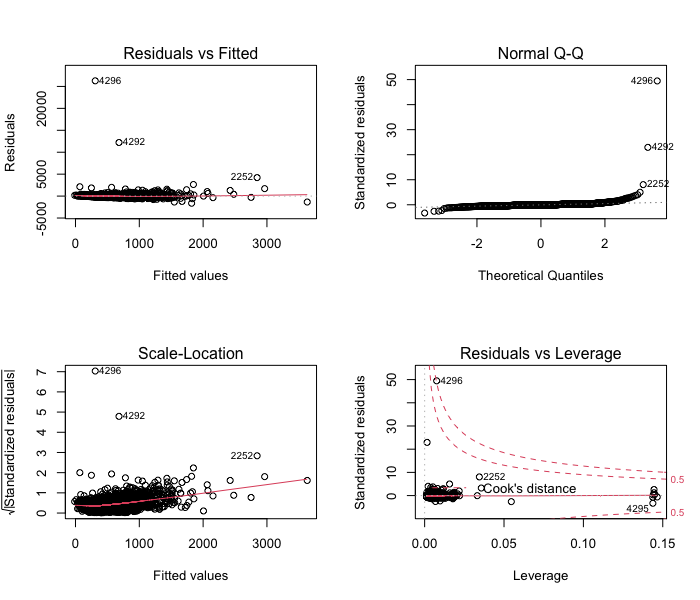
\includegraphics{/Users/florentinagalliers/Google Drive/Harper/1-C7081/Asssesment/github-C7081/C7081-assessment/diagnostic-plots.png}
Comparing the RMSE shown to the standard deviation of the price
variable..

\hypertarget{conclusions}{%
\subsection{Conclusions:}\label{conclusions}}

In the case of this dataset, a LASSO model containing 34 gave the lowest
RMSE. However a similarly acceptable low score was given by a multiple
linear regression containing only 15 variables which is much easier to
interpret due to it containing less variables. The predictor variables
that had the largest influence on House Price in this dataset were house
size (sqft\_living), number of bedrooms and bathrooms and house age. By
looking at the coefficients produced by the various models it is clear
that some of the location dummy variables had large impacts, in
particular houses in Seattle, Mercer Island, Medina and Bellevue had
more expensive homes, and those in Federal Way had less expensive homes.
Seattle is the capital city of Washington and so this may be an
explanation of the higher house prices, if it a more popular place to
live.

By using a larger data set, more accurate models may be possible. It was
clear location had a large impact, so potentially by focusing on one
smaller area the model could be refined for the other non-location
variables. Some of the city factor levels only contained information for
a small number of houses, and others (e.g.~Seattle) contained over
1,000, this may have influenced their influence on the price variable in
this dataset.

Overall, the linear regression model containing only 15 variables proved
to be easily interpretable and gave one of the lowest RMSE scores.
RandomForests produced RMSE scores in the same region as a linear model
containing only one variable, this suggests that they can be useful if
there are fewer variables.

\hypertarget{references}{%
\section*{References}\label{references}}
\addcontentsline{toc}{section}{References}

\hypertarget{refs}{}
\leavevmode\hypertarget{ref-alfiyatin2017modeling}{}%
Alfiyatin, Adyan Nur, Ruth Ema Febrita, Hilman Taufiq, and Wayan Firdaus
Mahmudy. 2017. ``Modeling House Price Prediction Using Regression
Analysis and Particle Swarm Optimization.'' \emph{International Journal
of Advanced Computer Science and Applications} 8.

\leavevmode\hypertarget{ref-bin2004prediction}{}%
Bin, Okmyung. 2004. ``A Prediction Comparison of Housing Sales Prices by
Parametric Versus Semi-Parametric Regressions.'' \emph{Journal of
Housing Economics} 13 (1): 68--84.

\leavevmode\hypertarget{ref-gao2019location}{}%
Gao, Guangliang, Zhifeng Bao, Jie Cao, A Kai Qin, Timos Sellis, Zhiang
Wu, and others. 2019. ``Location-Centered House Price Prediction: A
Multi-Task Learning Approach.'' \emph{arXiv Preprint arXiv:1901.01774}.

\leavevmode\hypertarget{ref-lu2017hybrid}{}%
Lu, Sifei, Zengxiang Li, Zheng Qin, Xulei Yang, and Rick Siow Mong Goh.
2017. ``A Hybrid Regression Technique for House Prices Prediction.'' In
\emph{2017 Ieee International Conference on Industrial Engineering and
Engineering Management (Ieem)}, 319--23. IEEE.

\end{document}
